\documentclass[12pt,a4paper]{article}

% --- Préambule : Configuration du document ---
\usepackage[utf8]{inputenc}
\usepackage[T1]{fontenc}
\usepackage[french]{babel}
\usepackage{graphicx}
\usepackage{geometry}
\usepackage{float}
\usepackage{hyperref}

% Marges
\geometry{hmargin=2.5cm,vmargin=2.5cm}

% Page de garde
\title{Travail Pratique \#1 : Modèles de langue et classification \\ \large IFT-4022/IFT-7022 Traitement automatique de la langue naturelle}
\author{Valentin Joncheray}
\date{Automne 2026 \\ Université Laval}

% --- Début du document ---
\begin{document}
	
	\maketitle
	
	\section{Tâche 2 : Classification de textes - Découvrez les classes d'incidents}
	
	\subsection{Méthodologie et Évaluation des Modèles}
	Dans cette section, nous comparons les performances de deux algorithmes pour classifier des descriptions d'incidents de chantiers de construction : le Naïf Bayésien (NB) et la Régression Logistique (LR).
	
	Les résultats obtenus sur les données de test sont les suivants :
	\begin{itemize}
		\item \textbf{Naïf Bayésien :} Exactitude (Accuracy) de 67,6 \% sur les données de test (85,7 \% à l'entraînement).
		\item \textbf{Régression Logistique :} Exactitude (Accuracy) de 69,3 \% sur les données de test (100,0 \% à l'entraînement).
	\end{itemize}
	
	\begin{figure}[H]
		\centering
		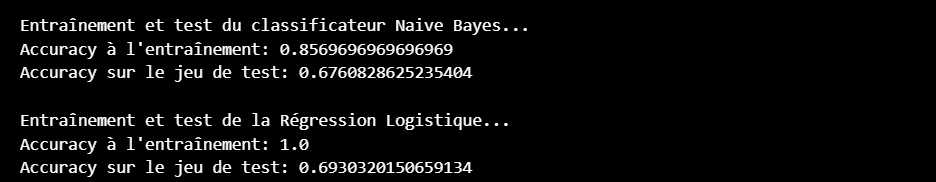
\includegraphics[width=0.7\textwidth]{results.png}
		\caption{Comparaison des résultats d'exactitude (Accuracy) entre les modèles.}
		\label{fig:results}
	\end{figure}
	
	Bien que la Régression Logistique montre un surapprentissage important (100 \% sur les données d'entraînement), elle généralise légèrement mieux sur les données de test que le Naïf Bayésien. C'est donc ce modèle qui a été retenu comme étant le plus performant pour notre analyse d'explicabilité.
	
	\begin{figure}[H]
		\centering
		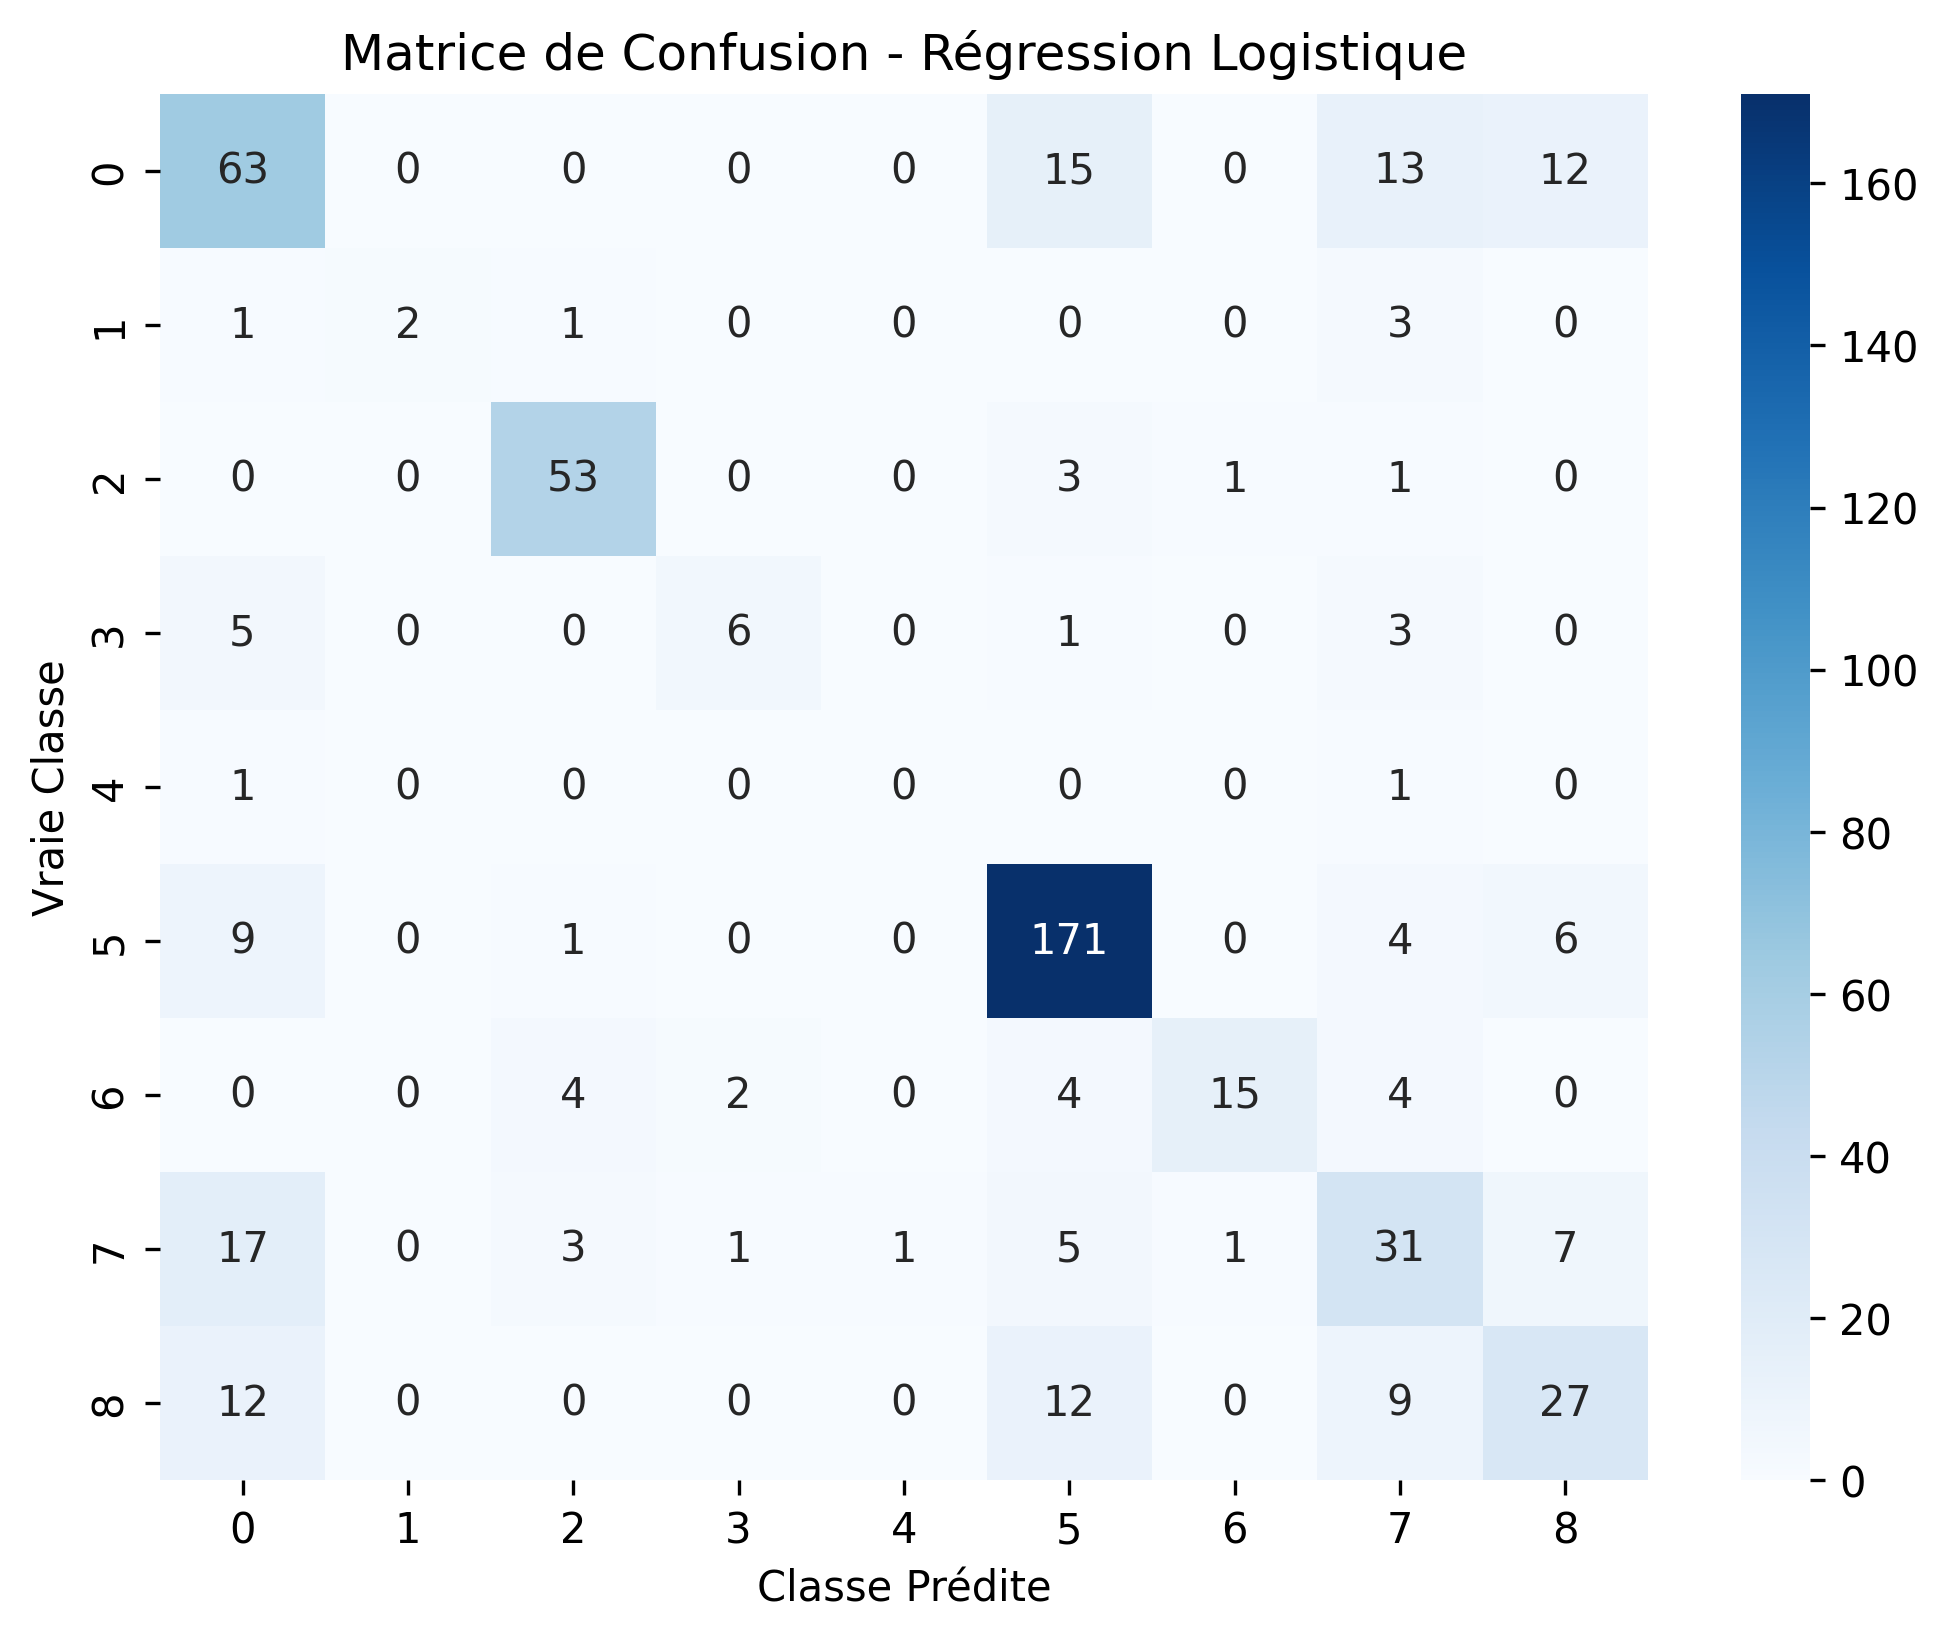
\includegraphics[width=0.7\textwidth]{matrice_lr.png} 
		\caption{Matrice de confusion du modèle de Régression Logistique sur les données de test.}
		\label{fig:confusion_lr}
	\end{figure}
	
	\subsection{Explicabilité et Interprétation des Classes}
	Afin de déterminer à quoi correspond chacune des classes d'incidents (initialement numérotées de 0 à 8), nous avons analysé les poids (\textit{coef\_}) du modèle de Régression Logistique ainsi que les probabilités du Naïf Bayésien. 
	
	\begin{figure}[H]
		\centering
		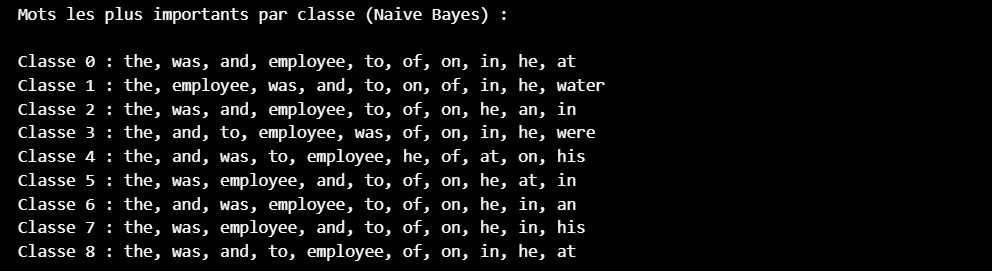
\includegraphics[width=0.8\textwidth]{Vecteur NB.png}
		\caption{Mots les plus importants par classe selon le modèle Naïf Bayésien (dominé par les mots de liaison).}
		\label{fig:vecteur_nb}
	\end{figure}
	
	\begin{figure}[H]
		\centering
		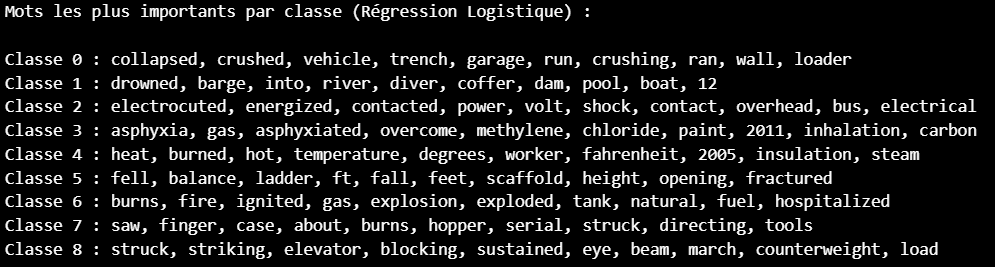
\includegraphics[width=0.8\textwidth]{Vecteur LR.png}
		\caption{Mots les plus importants par classe selon le modèle de Régression Logistique (vocabulaire discriminant).}
		\label{fig:vecteur_lr}
	\end{figure}
	
	Comme l'illustrent les figures \ref{fig:vecteur_nb} et \ref{fig:vecteur_lr}, les deux modèles extraient des mots radicalement différents. Cette disparité s'explique par leur fonctionnement mathématique :
	
	\begin{itemize}
		\item \textbf{Le Naïf Bayésien se base sur la fréquence absolue (probabilités pures) :} Cet algorithme calcule quels mots apparaissent le plus souvent dans une classe donnée. Lors de l'étape de vectorisation, nous n'avons pas retiré les mots de liaison (\textit{stop words} comme \textit{the, and, was, employee}). Par conséquent, ces mots très courants dominent naturellement le classement de chaque classe, car ils sont tout simplement les plus utilisés dans la langue anglaise, peu importe le type d'incident.
		\item \textbf{La Régression Logistique cherche la discrimination :} Cet algorithme attribue des «~poids~» aux mots pour maximiser sa capacité à distinguer une classe d'une autre. Un mot comme \textit{the} apparaît dans la classe "Noyade" autant que dans la classe "Chute", il n'aide donc pas le modèle à trancher ; la régression logistique lui donne alors un poids très faible (proche de zéro). À l'inverse, un mot comme \textit{electrocuted} est un indice exclusif à la classe 2 : le modèle lui attribue donc un poids positif massif.
	\end{itemize}
	
	Voici donc l'interprétation déduite de l'analyse des mots discriminants (Régression Logistique) pour chaque classe :
	
	\begin{itemize}
		\item \textbf{Classe 0 - Éboulement / Écrasement :} \textit{collapsed, crushed, trench, crushing, wall}
		\item \textbf{Classe 1 - Noyade :} \textit{drowned, river, diver, pool, boat}
		\item \textbf{Classe 2 - Électrocution :} \textit{electrocuted, energized, power, volt, shock}
		\item \textbf{Classe 3 - Asphyxie / Gaz :} \textit{asphyxia, gas, asphyxiated, inhalation, carbon}
		\item \textbf{Classe 4 - Brûlures thermiques :} \textit{heat, burned, hot, temperature, steam}
		\item \textbf{Classe 5 - Chutes de hauteur :} \textit{fell, balance, ladder, fall, scaffold}
		\item \textbf{Classe 6 - Incendies / Explosions :} \textit{burns, fire, ignited, explosion, exploded}
		\item \textbf{Classe 7 - Blessures avec outils / Amputations :} \textit{saw, finger, tools, struck, amputated}
		\item \textbf{Classe 8 - Heurté par un objet / Charge lourde :} \textit{struck, elevator, beam, counterweight, load}
	\end{itemize}
	
	L'approche discriminatoire de la Régression Logistique a ainsi permis d'isoler le vocabulaire métier spécifique à chaque type d'incident et de lever le voile sur les étiquettes numériques du jeu de données.
	
\end{document}